\chapter{Analisis}
\label{chap:analisis}

\section{Analisis Perangkat Lunak Sejenis}
\label{sec:analisis pl}

Salah satu \textit{website} yang dapat memberikan rekomendasi program studi adalah \url{https://rencanamu.id}. \textit{Website} tersebut dikembangkan menggunakan riset ilmiah, Rencanamu mengukur 7 dimensi profil siswa sebagai landasan dalam rekomendasi, perencanaan kuliah dan karier yang terintegrasi, berkesinambungan dan menyeluruh. Gambar \ref{gambar31} menunjukkan 7 dimensi profil siswa. % https://rencanamu.id/about-us

\begin{figure}[H]
    \centering
    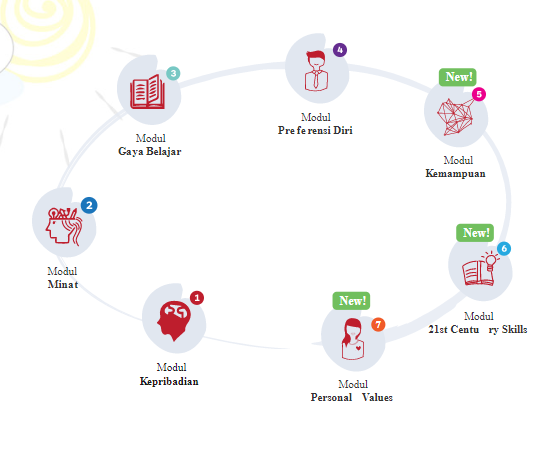
\includegraphics[width = 10cm, height = 10cm]{doc/DokumenSkripsi/Gambar/gambar31.PNG}
    \caption{7 Dimensi Profil Siswa}
    \label{gambar31}
\end{figure}

Pada \textit{website} ini, telah dilakukan beberapa analisis dan hasilnya sebagai berikut :

\begin{enumerate}
    \item \textit{Website} \url{https://rencanamu.id} adalah sebuah \textit{platform} persiapan kuliah dan karier \textit{online} berbasis data didukung oleh teknologi \textit{People Science} untuk membantu siswa dalam merancang dan mempersiapkan masa depan mereka. 
    
    \item Perlu melakukan registrasi atau \textit{login} kedalam \textit{website}.
    
    \item Gambar \ref{gambar32} merupakan tampilan awal setelah registrasi atau \textit{login}.
    
    \begin{figure}[H]
        \centering
        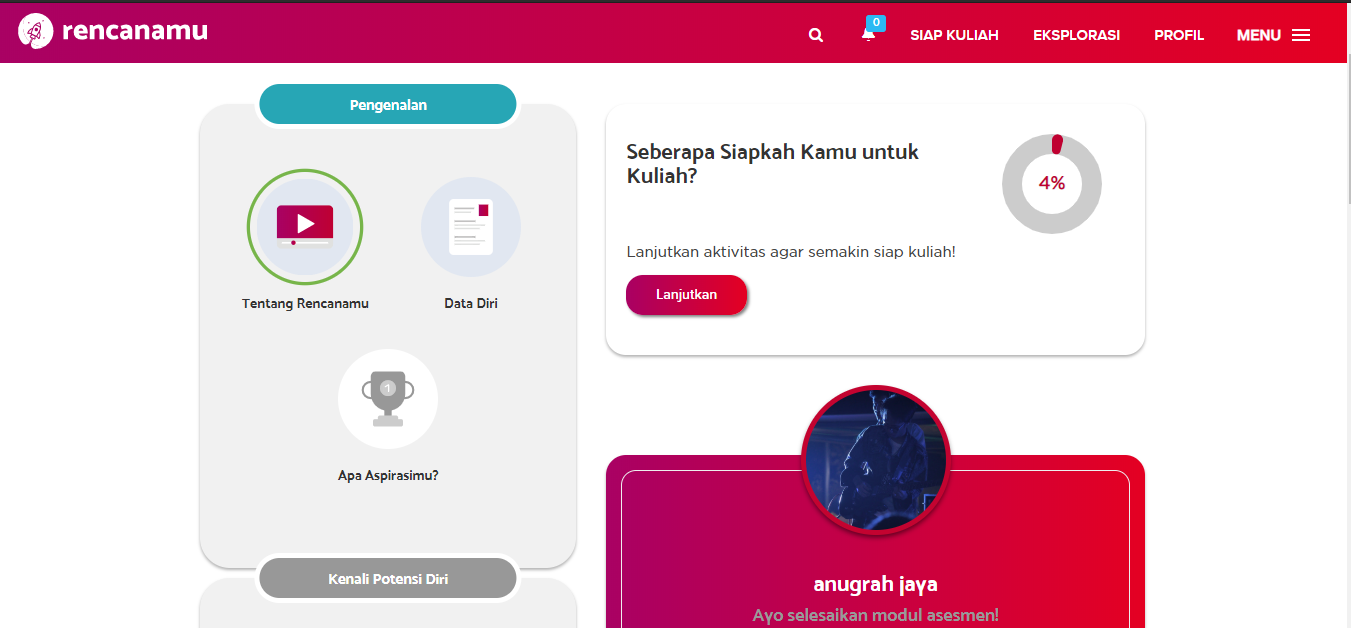
\includegraphics[width = 8cm, height = 5 cm]{doc/DokumenSkripsi/Gambar/gambar32.PNG}
        \caption{Tampilan setelah registrasi atau \textit{login}}
        \label{gambar32}
    \end{figure}
    
    \item Gambar \ref{gambar33}, Gambar \ref{gambar34}, dan Gambar \ref{gambar35} adalah beberapa modul yang harus dikerjakan.
    
    \begin{figure}[H]
        \centering
        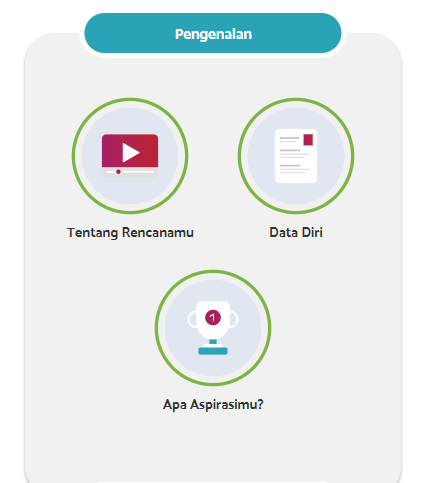
\includegraphics[width = 6cm, height = 7cm ]{doc/DokumenSkripsi/Gambar/gambar33.PNG}
        \caption{Caption}
        \label{gambar33}
    \end{figure}
    
    \begin{figure}[H]
        \centering
        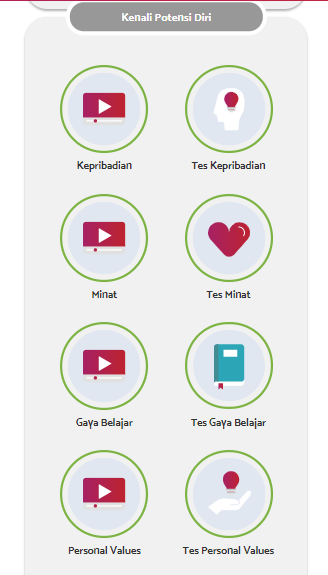
\includegraphics[width = 6cm, height = 9cm ]{doc/DokumenSkripsi/Gambar/gambar34.PNG}
        \caption{Caption}
        \label{gambar34}
    \end{figure}
    
    \begin{figure}[H]
        \centering
        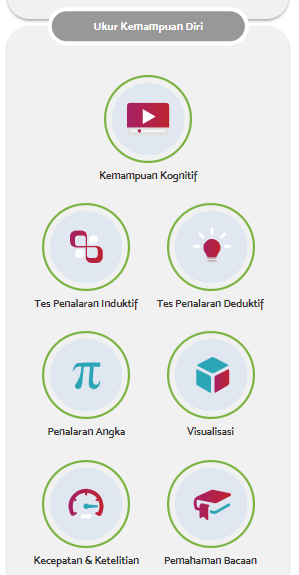
\includegraphics[width = 6cm, height = 8cm ]{doc/DokumenSkripsi/Gambar/gambar35.PNG}
        \caption{Caption}
        \label{gambar35}
    \end{figure}
    
    \item Gambar \ref{gambar36} adalah contoh hasil rekomendasikan yang diberikan sistem berdasarkan modul yang sudah dikerjakan.
    
    \begin{figure}[H]
        \centering
        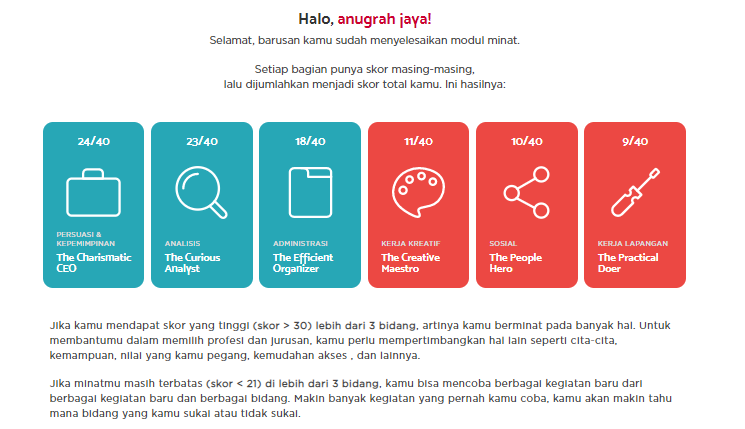
\includegraphics[width = 7cm, height = 8cm ]{doc/DokumenSkripsi/Gambar/gambar36.PNG}
        \caption{Hasil Rekomendasi}
        \label{gambar36}
    \end{figure}
    
\end{enumerate}

\textit{Website} \url{https://rencanamu.id} memiliki kesamaan dengan \textit{website} yang dibangun yaitu memberikan rekomendasi program studi untuk anak SMA. Perbedaannya pada \textit{website} \url{https://rencanamu.id} tidak menampilkan prediksi IPK dan harus mengisi beberapa modul untuk mendapatkan rekomendasi program studi. 

\section{Pemilihan Algoritma Sistem Rekomendasi}
Berdasarkan teori \ref{teknik rekomendasi} yang menjelaskan mengenai teknik-teknik yang dapat digunakan untuk membangun sistem rekomendasi, teknik \textit{collaborative filtering} adalah teknik yang dapat digunakan untuk memberikan rekomendasi berupa program studi kepada calon mahasiswa berdasarkan kesamaan dengan pengguna lain. Berikut merupakan beberapa hal mengapa memilih teknik \textit{collaborative filtering} :

\begin{enumerate}
    \item \textit{Collaborative filtering} menghasilkan rekomendasi item yang spesifik untuk pengguna berdasarkan peringkat tanpa memerlukan informasi tambahan mengenai item ataupun pengguna.
    
\end{enumerate}

Teknik \textit{collaborative filtering} memiliki beberapa kekurangan diantaranya : 

\begin{enumerate}
    \item Rekomendasi yang diberikan mengambil data yang cukup banyak dari basis data sehingga membutuhkan memori yang besar.
    
    \item Tidak bisa memberikan rekomendasi untuk item yang tidak pernah diberikan \textit{rating} oleh pengguna.
    
    \item Pengguna harus memberikan \textit{rating} untuk beberapa atribut agar bisa diberikan rekomendasi.
    
\end{enumerate}

Pada \textit{website} yang dibangun, akan memberikan rekomendasi berdasarkan nilai raport beberapa mata pelajaran siswa pada kelas 10 dan 11 yang digunakan untuk PMDK. Mata pelajaran yang digunakan adalah Matematika, Bahasa Indonesia, Bahasa Inggris, Fisika, Kimia, dan Pendidikan Kewarganegaraan. Rekomendasi program studi berdasarkan asal jurusan saat SMA, misalnya siswa IPA akan diberikan rekomendasi program studi IPA.

\section{\textit{Preprocessing} Data Mahasiswa}
\label{sec:preprocessing}
Data mahasiswa yang digunakan adalah data mahasiswa Universitas Katolik Parahyangan dengan jalur penerimaan Penelurusan dan Kemampuan atau PMDK pada tahun 2013-2018. Pada data yang digunakan terdapat beberapa atribut yang tidak dapat digunakan seperti No.PMB,  kota asal sekolah, dan provinsi asal sekolah. Atribut yang tidak dapat digunakan akan dihapus dan data akan dipisahkan menjadi dua \textit{file} mahasiswa dan nilai untuk setiap program studi yang ada. \textit{prepocessing} dilakukkan menggunakan Python. Berikut langkah-langkah dalam \textit{preprocessing} :

\begin{enumerate}
    \item Membaca file .csv yang berisikan data mahasiswa pada fakultas tertentu.
    
    \item Membuat dataframe untuk menampung data mahasiswa dan nilai.
    
    \item Menginisialisasikan batas \textit{looping}, id\_user, id\_nilai, dan asal jurusan.
    
    \item Menambahkan data mahasiswa berupa NPM, id\_prodi, asal jurusan, dan IPK pada dataframe mahasiswa.
    
    \item Mengubah \textit{range} nilai menjadi GPA (\textit{Grade Point Average}) dan menghitung nilai rata-rata untuk setiap nilai mata pelajaran.
    
    \item Menambahkan data GPA, rata-rata nilai, dan id\_user pada dataframe nilai.
    
    \item Menyimpan dataframe mahasiswa dan nilai menjadi .csv.
\end{enumerate}

\section{Contoh Perhitungan Pearson Correlation}
Berdasarkan \ref{user-based} terdapat langkah-langkah perhitungan dari \textit{user-based}. Tabel \ref{tab:data mahasswa} merupakan contoh data mahasiswa.

\begin{table}[H]
    \centering
    \begin{tabular}{|l|c|c|c|c|c|}
        \hline
        MP\slash Semester & 101 & 102 & 111 & 112 & AVG \\
        \hline 
        Matematika & 2.6 & 2.9 & 2.95 & 2.75 & 2.8 \\
        \hline 
        Bahasa Indonesia & 0 & 0 & 0 & 0 & 0 \\
        \hline 
        Bahasa Inggris & 2.95 & 3 & 2.85 & 2.95 & 2.9375 \\
        \hline 
        PKN & 0 & 0 & 0 & 0 & 0 \\
        \hline
    \end{tabular}
    \caption{Contoh data mahasiswa dalam bentuk GPA}
	\label{tab:data mahasswa}
\end{table}

Berikut merupkan contoh langkah-langkah perhitungan :

\begin{enumerate}
    \item Menghitung nilai rata-rata \textit{rating}.
    
    \begin{table}[H]
    \centering
    \begin{tabular}{|l|c|c|c|c|c|c|}
        \hline
        MP\slash Semester & 101 & 102 & 111 & 112 & Rumus & AVG \\
        \hline 
        Matematika & 2.9 & 3.4 & 3.4 & 2.9 & $\frac{2.9 + 3.4 +3.4 + 2.9}{4}$ & 3.15 \\
        \hline 
        Bahasa Indonesia & 2.95 & 2.9 & 3.9 & 3.4 & $\frac{2.95 + 2.9 + 3.9 + 3.4}{4}$ & 3.2875 \\
        \hline 
        Bahasa Inggris & 3.3 & 3.35 & 3.25 & 2.9 & $\frac{3.3 + 3.35 + 3.25 + 2.9}{4}$ & 3.2 \\
        \hline 
        PKN & 3.4 & 2.9 & 3.35 & 2.35 & $\frac{3.4 + 2.9 + 3.35 + 2.35}{4}$ & 3 \\
        \hline
    \end{tabular}
    \caption{Contoh data siswa dalam bentuk GPA}
	\label{tab:data siswa}
\end{table}

    \item Menghitung kesamaan atau similaritas.
    
    \begin{table}[H]
        \centering
        \begin{tabular}{|c|c|c|c|c|}
            \hline
            No & Rumus & Matematika & Rumus & Bahasa Inggris \\
            \hline
            \multirow{2}{*}{1} & $(2.9-3.15)*$ & 0.5    & $(3.3-3.2)*$ & 0.00125\\
            & $(2.6-2.8)$ & & $(2.95-2.9375)$ &  \\
            \hline
            \multirow{2}{*}{2} & $(3.4-3.15)*$ & 0.025  & $(3.35-3.2)*$ & 0.009375 \\
            & $(2.9-2.8)$ & & $(3-2.9375)$ &  \\
            \hline
            \multirow{2}{*}{3} & $(3.4-3.15)*$ & 0.0375 & $(3.25-3.2)*$ & -0.004375 \\
            & $(2.95-2.8)$ &  & $(2.85-2.9375)$ &  \\
            \hline
            \multirow{2}{*}{4} & $(2.9-3.15)*$ & 0.0125 & $(2.9-3.2)*$ & -0.00375 \\
            & $(2.75-2.8)$ &  & $(2.95-2.9375)$ &  \\
            \hline
            \multirow{2}{*}{Sigma} & $0.5 + 0.025 +$ & 0.125 & $0.00125 + 0.009375 +$ & 0.0025 \\
            & $0.0375 + 0.0125$ & & $-0.004375 + -0.00375$ &  \\
            \hline
            \multicolumn{3}{|c|}{Hasil} & $0.125+0.0025$ & 0.1274 \\
            \hline
        \end{tabular}
        \caption{Nilai kovariasi mahasiswa dan siswa}
        \label{tab:kovariasi}
    \end{table}
    
    \item Memilih nilai kesamaan atau similaritas yang bernilai lebih dari 0.
    
    \item Menghitung nilai prediksi.
\end{enumerate}

\section{\textit{Framework}}

\subsection{\textit{Framework} Laravel}

\subsection{\textit{Framework} Bootstrap}

\section{Analisis Kebutuhan Sistem}

\subsection{Rancangan Basis Data}
% erd, table, skema relasi

% perlu atau engga ? kata bu mar ga terlalu perlu
\subsection{Diagram \textit{Use-Case}}

